\documentclass[../main.tex]{subfiles}
%\usepackage{algorithm}
%\usepackage{algorithmic}


\everymath{\displaystyle}
\def\arraystretch{2.0}
\def\naca0012path{/home/lukas/Desktop/project/independence/project/simulations/naca0012}
\begin{document}
\setlength{\delimitershortfall}{0pt}

\FloatBarrier 
\chapter{Examples}\label{sec:examples}
\minitoc
%\sectlof
%\sectlot


This section is denoted to simple examples of the newly implemented analytic sensitivity framework. Due to a limited time available, we restricted our considerations to simple 2D problems. Particularly, an optimization on the NACA0012 profile, as already described in figure~\ref{fig:verification_setup}, is presented in section~\ref{sec:example_naca}.\\
A slightly more cumbersome example, that nicely portrays the advantages of the embedded sensitivity framework is then provided in section \ref{sec:example_multielem}. Here, the flap and slats configuration of an airfoil is maximized. This requires large deformations and would not be possible with the body-fitted sensitivity framework.

\section{\ac{LDR} shape-optimization of a NACA0012 airfoil}\label{sec:example_naca}
We consider the optimization of a NACA0012 airfoil for an angle of attack of $\alpha=0.0^{\circ}$ and a Mach number of 0.3. %For comparison, both the inviscid and the viscous results are provided.


\subsection{Setup}\label{sec:naca0012_setup}
The setup has already been described in figure~\ref{fig:verification_setup}. The shape is described using the design variable concept (see section~\ref{sec:design_model}) with $8$ abstract variables.
In this particular example, the lower, front design variable has been fixed in order to prevent rigid body motions.
\subsection{Results}\label{sec:naca0012_results}

The example has been run meshed with $\sim1000000$ nodes and running on 60 compute cores. All forces have been evaluated on the discrete embedded surface. Both the initial and the final, converged shape are provided in figure \ref{fig:naca0012_ldr_solutions}.



\begin{figure}[t!]
    \centering
    	\begin{subfigure}[t]{0.45\textwidth}
    	\includegraphics[width=\linewidth]{\mainpath/fig/tikz/build/naca0012_optimization_convergence.pdf}
    	\caption{Convergence}
    	\end{subfigure}
    	\begin{subfigure}[t]{0.45\textwidth}
    	\includegraphics[width=\linewidth]{\naca0012path/minLiftOverDrag/mesh/archive/euler_frontfixed_9it_nominlift/py/surfaces_borderless.pdf}
    	\caption{shapes}
    	\end{subfigure}
    	\caption[NACA0012 LDR optimization - convergence]{Convergence of the \ac{LDR} during the optimization. A \ac{BFGS} algorithm has been used for optimization. The left figure shows the convergence of the lift-to-drag ratio, the right figure displays the different airfoil shapes during the optimization process.}
    \label{fig:nac0012_ldr_convergence}
\end{figure}

%\naca0012path/minLiftOverDrag/mesh/archive/euler_frontfixed_9it_nominlift/py/surfaces_borderless.pdf


\begin{figure}[t!]
    \centering
    	\begin{subfigure}[t]{0.40\textwidth}
    	    \setlength{\fboxsep}{\valfboxsep}%\valfboxsep=0pt
        \setlength{\fboxrule}{\valfboxrule}%\valfboxrule=1pt
			  \fbox{\includegraphics[width=\linewidth]{\naca0012path/minLiftOverDrag/mesh/euler2/post/png/It000_velx.png}}
			  %\caption{NACA0012 original shape}
		\end{subfigure}\hfill~
    	\begin{subfigure}[t]{0.40\textwidth}
    	    	\setlength{\fboxsep}{\valfboxsep}%\valfboxsep=0pt
        \setlength{\fboxrule}{\valfboxrule}%\valfboxrule=1pt
			  \fbox{\includegraphics[width=\linewidth]{\naca0012path/minLiftOverDrag/mesh/euler2/post/png/It009_velx.png}}
			  %\caption{final optimized shape}
		\end{subfigure}~
    	\begin{subfigure}[t]{0.1\textwidth}
			  \includegraphics[scale=0.40]{\naca0012path/minLiftOverDrag/mesh/euler2/post/png/colorbar_velocity.png}
			  %\caption{final optimized shape}
		\end{subfigure}\\\vspace{1cm}
    	\begin{subfigure}[t]{0.40\textwidth}
    	    \setlength{\fboxsep}{\valfboxsep}%\valfboxsep=0pt
        \setlength{\fboxrule}{\valfboxrule}%\valfboxrule=1pt
			  \fbox{\includegraphics[width=\linewidth]{\naca0012path/minLiftOverDrag/mesh/euler2/post/png/It000_press.png}}
			  \caption{NACA0012 original shape}
		\end{subfigure}\hfill~
    	\begin{subfigure}[t]{0.40\textwidth}
    	    \setlength{\fboxsep}{\valfboxsep}%\valfboxsep=0pt
        \setlength{\fboxrule}{\valfboxrule}%\valfboxrule=1pt
			  \fbox{\includegraphics[width=\linewidth]{\naca0012path/minLiftOverDrag/mesh/euler2/post/png/It009_press.png}}
			  \caption{final optimized shape}
		\end{subfigure}~
    	\begin{subfigure}[t]{0.1\textwidth}
			  \includegraphics[scale=0.40]{\naca0012path/minLiftOverDrag/mesh/euler2/post/png/colorbar_press.png}
			 % \caption{final optimized shape}
		\end{subfigure}
    \caption[NACA0012 LDR optimization - solution fields]{Lift over Drag optimization of a 2D airfoil in the embedded framework. The design element configuration of the embedded surface is depicted in Figure~\ref{fig:verification_setup}.}
    \label{fig:naca0012_ldr_solutions}
\end{figure}


%\pgfplotstableread[col sep = comma]{/home/lukas/Desktop/project/independence/project/simulations/naca0012/minLiftOverDrag/mesh/archive/euler_frontfixed_9it_nominlift/py/LDR.csv}\mydata
%\begin{tikzpicture}
% \addplot table[y = 1st col]{\mydata};
%\end{tikzpicture}


\section{Multi-element airfoil with large kinematics}\label{sec:example_multielem}

The second example aims at pointing out the superiority of the embedded approach over the body-fitted approach when it comes to shape optimization. Due to the large motions involved, this example would not have been possible with a body-fitted framework. The setup is described in section~\ref{sec:multielem_setup} and the results are presented in section~\ref{sec:multielem_results}.

\subsection{Setup}\label{sec:multielem_setup}

The setup is described in figure~\ref{fig:multi_elem_setup}. The airfoil consists of 3 separate parts, where the front and back can perform large motions. Each motion is described by a single parameter(rotatory movement). This way, the parameter space has been kept low-dimensional, which enabled us to sample the whole space, thereby verifying that the optimizer indeed finds the correct solution

\begin{figure}[t!]
    \centering
    	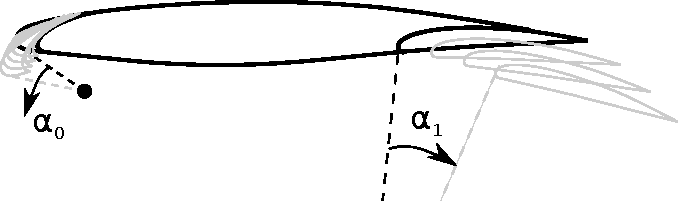
\includegraphics[width=0.5\linewidth]{/home/lukas/Desktop/project/independence/project/thesis/fig/pdf/multielem/setup.pdf}
    	\caption[Multi-element example: setup]{Setup for the multi-element example. A 3 element airfoil is considered. The motion of the from of back element is being described via a simple rotation. This is done on purpose to keep the parameter-space low-dimensional. This example would not be possible in the body-fitted framework.}
    	\label{fig:multi_elem_setup}
\end{figure}


\subsection{Results}\label{sec:multielem_results}
The objective of this simulation was the minimization of the lift over drag ratio. We prescribed both minimum lift and maximum drag constraints. The optimization was then performed using an \ac{SLSQP} algorithm. In order to verify the results of the optimizer, we performed a $30\times30$ sampling of the parameter space. The lift and drag results are visualized in figure~\ref{fig:multi_elem_liftanddrag} and the lift over drag ration is printed over the parameter space in figure~\ref{fig:multi_elem_ldr}.

\begin{figure}[t!]
    \centering
    	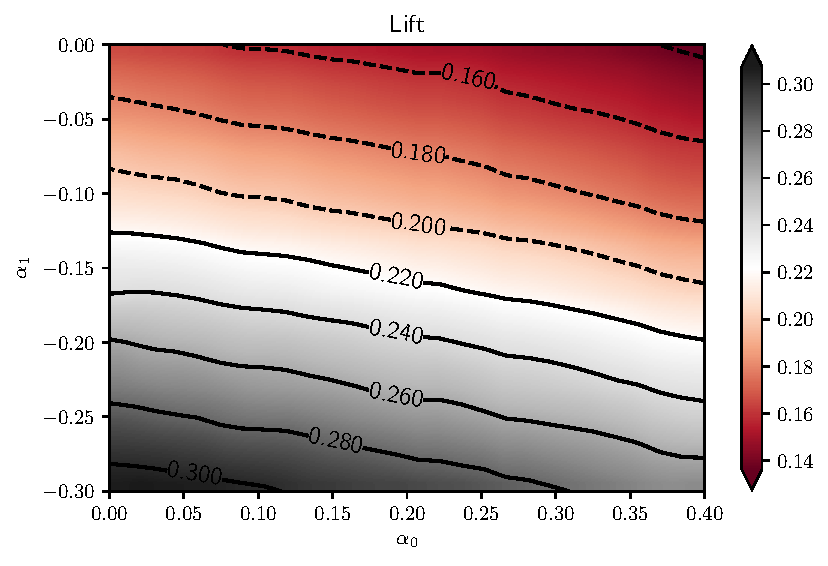
\includegraphics[width=0.5\linewidth]{\mainpath/fig/pdf/multielem/lift.pdf}~
    	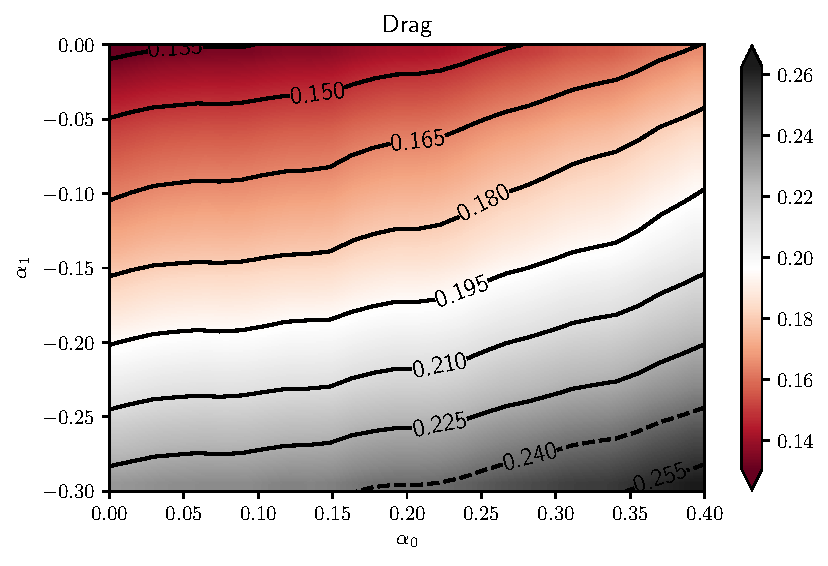
\includegraphics[width=0.5\linewidth]{\mainpath/fig/pdf/multielem/drag.pdf}
    	\caption[Multi-element example: lift and drag]{Lift(left figure)- and drag(right figure)- results plotted over the parameter space spanned by $\alpha_0$ and $\alpha_1$. ISO-lines that don't fulfill the minimum lift or maximum drag requirements are plotted in dashed lines. An optimum is searched in the remaining parameter space. The optimum found is plotted in figure~\ref{fig:multi_elem_ldr}}
    	\label{fig:multi_elem_liftanddrag}
\end{figure}

\begin{figure}[t!]
    \centering
    	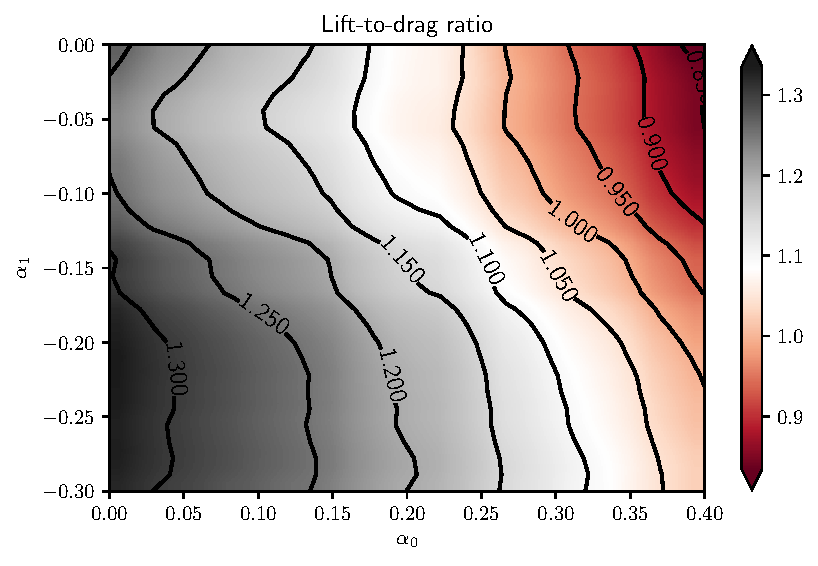
\includegraphics[width=0.5\linewidth]{\mainpath/fig/pdf/multielem/liftdrag.pdf}
    	\caption[Multi-element example: LDR-ratio]{\acf{LDR} over the parameter space for the example presented in figure~\ref{fig:multi_elem_setup}. $\alpha_0$ id plotted over the horizontal axis, $\alpha_1$ over the vertical axis. There is no local maximum, instead the optimum is on the border of the parameter space. Both the starting configuration as well as the optimum found by the optimizer are plotted. The optimization has been perfomed using \texttt{SciPy:L-BFGS-B}. }
    	\label{fig:multi_elem_ldr}
\end{figure}




\end{document}





